We use \textit{precision} and \textit{recall} to evaluate our models. 
In practice, each article which produces a high number of comments is more likely to bind resources of comment moderators and editors.
Therefore, a high classification \textit{precision} is important as well as a high \textit{recall} to omit as few classifications as possible.
\textit{Precision} and \textit{recall} are equally relevant and consequently, we use the harmonic mean, the $F_1$-score, of both metrics. As \textit{precision}, \textit{recall}, and the $F_1$-score are common metrics for binary classification problems, it is possible to compare our results against those of existing approaches.

\subsection{Model Performances}
An overview of our results in \autoref{tbl:results_basic} depicts that all our models reach a significantly higher \textit{recall} than \textit{precision}.

\textit{Model 3} reaches the highest \textit{precision} with a value of $0.228$, and \textit{Model 7} the highest \textit{recall} with a value of $0.917$. \textit{Model 4} achieves the highest $F_1$-score of $0.330$. 

% Table 3: Precision (P), recall (R), and F1-score of the baseline, all article and metadata features, annotations of comments shown on the first page, and all combined.
\begin{table}[h]
	\centering
	\caption{\textmd{Precision (P), recall (R), and $F_1$-score of all basic models.}}
	\label{tbl:results_basic}
	\vspace{-0.2cm}
	\begin{tabular}{cllccc}
		\toprule
		% \textbf{Features} &
		\specialcellbold{ID} &
		\specialcellbold{Input} &
		\specialcellbold{Type} &
		\specialcellbold{P} &
		\specialcellbold{R} &
		\specialcellbold{F$_1$} \\
		\midrule
		1 & headline & FC & .216 & .606  & .309  \\
		2 & headline & CNN & .221 & .603  & .314  \\
		3 & article & LSTM  & .228 & .493  & .302  \\
		4 & category & FC & .227 & .603  & .320  \\
		5 & time & FC  & .100 & .457  & .155  \\
		6 & text metrics & FC  & .133 & .738  & .222  \\
		7 & competitive score & FC & .112 & .917  & .197  \\
		\bottomrule
	\end{tabular}
\end{table}

\textit{Model 1} and \textit{2} process the same input. Despite the fact that the second model has approximately a third of the weights in its hidden layers, both of these models perform similarly for all three metrics.
We assume that the convolutional network (\textit{Model 2}) can learn fewer features whilst having a greater generalization potential through its shared weights.

\textit{Model 3} takes the first $50$ words of the article text as input. 
We found that inputing more or even all words from an article does not improve the ability of this model to predict comment volume.
\textit{Model 3} gave lower \textit{recall} values while achieving slightly higher \textit{precision} in comparison to those seen with \textit{Model 1} and \textit{2}. 
The $F_1$-score is therefore, similar for these first three models.
This is probably due to the similar context complexity provided by the words of the headline and the first 50 words of the article.

\textit{Model 4} achieves the most promising results. 
Despite the low complexity of the input feature, these results can be justified by the distribution of the categories within the GACC. 
Articles assigned to the \textit{comment is free} category have a probability of $22.8\%$ to be a top article as illustrated in \autoref{fig:top_ten_category}. 
Classifying just these articles as a top article already leads to an $F_1$-score of $0.292$.
If we only classify articles within the four categories with the highest amount of top articles as a top article, we receive an $F_1$-score of $0.316$. 
This explains why \textit{Model 4} has such a hight $F_1$-score.

\begin{figure}[h]
	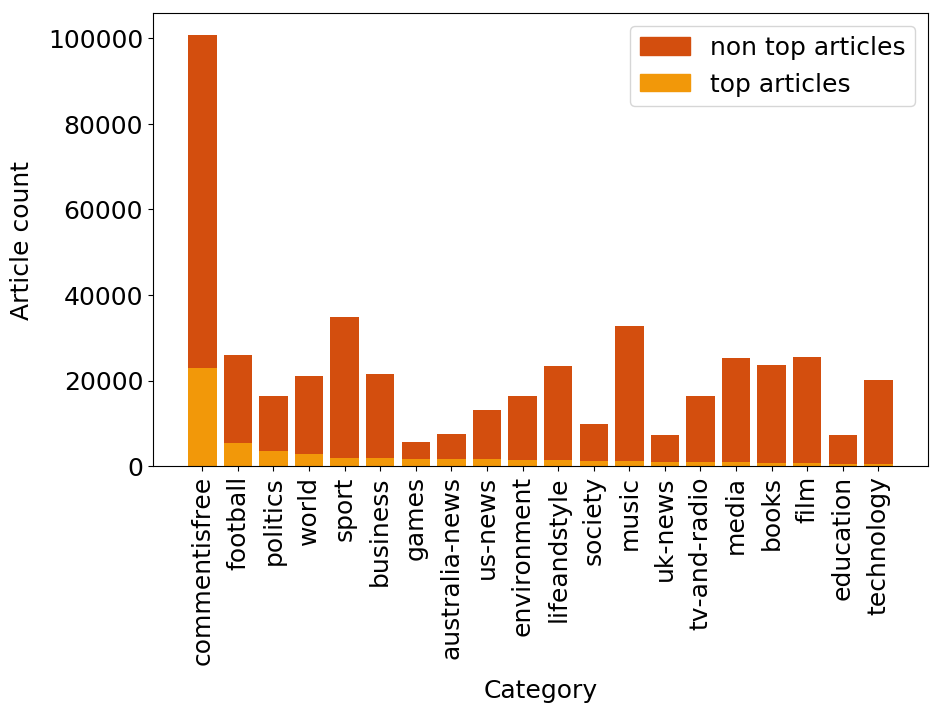
\includegraphics[width=0.4\textwidth]{fig/top_ten_category.png}
	\caption{\textmd{Number of articles for the first $20$ categories containing the most of the top articles.}}
	\label{fig:top_ten_category}
\end{figure}

\textit{Model 5} has a \textit{precision} value of $0.100$ which is the same as a random prediction.
It is possible that this is a result of $19\%$ of articles being released on full hours and also that \textit{The Guardian} has a readership spread located across multiple time zones.
Therefore, the time of the day has almost no effect on the number of comments that an article receives as seen in \autoref{fig:top_ten_time}. 
Additionally, the day of the week also has no significant effect on the weekly article performance. 

\begin{figure}[h]
	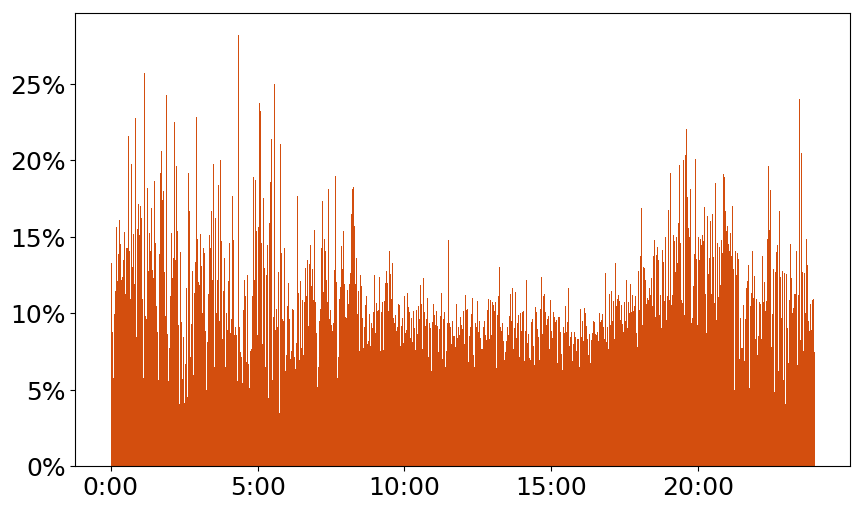
\includegraphics[width=0.4\textwidth]{fig/top_ten_time.png}
	\caption{\textmd{Percentage of top articles per time of the day.}}
	\label{fig:top_ten_time}
\end{figure}

\textit{Model 6} is slightly more effective than \textit{Model 5}. 
Neither the length of the headline nor the length of the article text is feasible for an accurate prediction.

\textit{Model 7} processes a single numeric value as input. 
For a good performance using the competitive score, it would be necessary to divide the values into distinct groups.
Unfortunately, the competitive score distribution of top articles is similar to that of all articles.

\subsection{Combined Models}
As seen in \autoref{fig:correlation_matrix}, \textit{Model 1} and \textit{2} correlate the most with a value of $0.589$ which is due to processing the same input feature.
The correlation between \textit{Model 3} and both models \textit{1} and \textit{2} is relatively high. 
This is probably due to the headline and the first $50$ words of the article which provide a similar context.

\autoref{tbl:results_combined} shows the results of our combinations. We combine \textit{Model 2} with each other model because it exhibits the best results processing text input and has a low correlation to other models.
\textit{Model 5} correlates least with the other models and has a low $F_1$-score. Therefore, we did not combine it with any other models.

\begin{table}[]
\centering
\label{tbl:results_combined}
\caption{\textmd{Precision (P), recall (R), and F$_1$-score of all combined models}}
\vspace{-0.2cm}\begin{tabular}{cccc}
\toprule
% \textbf{Features} &
% \specialcellbold{Short description} &
\specialcellbold{Combination} &
\specialcellbold{P} &
\specialcellbold{R} &
\specialcellbold{F$_1$} \\
\midrule
2 3 & .224 & .645 & .323\\
2 4 & .245 & .627 & .342\\
2 5 & .227 & .581 & .317 \\
2 6 & .217 & .651 & .317\\
2 7 & .214 & .625 & .311\\
3 4 & .252 & .577 & .339\\
2 3 4 & .265 & .607 & .357\\
\bottomrule
\end{tabular}
\end{table}

The combination of \textit{Model 2} with each of models \textit{5}, \textit{6}, and \textit{7} fails to perform better than \textit{Model 2} itself. 
This shows that, besides the headline text, the publishing time, text metrics, and competitive score are unnecessary to improve the comment volume prediction.

Combining each \textit{Model 3} and \textit{4} with \textit{Model 2} shows performance improvements. 
These combinations produced the best \textit{precision} and highest $F_1$-score.

Compared to the results of other approaches (\autoref{tbl:compare_approaches}), our $F_1$-score is $42\%$ higher than the value by Tsagikas et al.\ implemented by Ambroselli et al.\ and $5\%$ lower than the values obtained by Ambroselli et al.\ \cite{ambroselli2018prediction}.

\begin{table}[h]
\centering
\caption{\textmd{Precision (P), recall (R), and F$_1$-score of baseline approaches and our approach.}}
\label{tbl:compare_approaches}
\vspace{-0.2cm}\begin{tabular}{lccc}
\toprule
\specialcellbold{Approach} &
\specialcellbold{P} &
\specialcellbold{R} &
\specialcellbold{F$_1$} \\
\midrule
Tsagkias et al. & .16 & .72 & .26\\
Ambroselli et al. & .26 & .75 & .39\\
Our Approach & .27 & .61 & .37\\
\bottomrule
\end{tabular}
\end{table}

Finally, it is important to establish that our results were achieved using another dataset to that which Ambroselli et al.\ used for both approaches.
Their data contained only articles by a German magazine. 
\textit{The Guardian} releases its articles internationally which implies a much broader audience and meaning that topics are of a more diverse nature.
Tsagikas et al.\ took time features, metadata, e.g.\ article length, similar article count, several reference counts, e.g.\ count of referred people, and temperature data into account.
Ambroselli et al.\ additionally used publisher information such as the author and the editor.
To compare both approaches appropriately, it would be necessary to use the same dataset and the same range of features.

Further classification improvements could be achieved by using a more sophisticated network architecture. 
A recent approach taken by Conneau et al.\ shows that a very deep CNN architecture using character embeddings can be used for text classification \cite{conneau2016very}. 
Applying this method could lead to a more coherent semantic interpretation of the text features which would result in more precise prediction.